\section{Cached Sequential Comparison}
\label{sec:cached-comparison}
Both backends were measured again on the same host with the same Release
compiler flags, seed, and field as Section~\ref{sec:original-baseline}.
Each point represents three separate sequential processes, so the arithmetic
caches begin empty for each run. The whole-workload application interval includes
generation, matrix multiplication, the three determinants, and cache creation
and filling; it ends before static-cache destruction. Peak resident set size
(RSS) includes the cache. Builds and profiling were excluded from these timings.
All executions returned successfully, verified the determinant identity, and
matched the original determinant coefficients at their dimension.

Fig.~\ref{fig:backend-comparison} compares median application totals, the
ratio of original to cached medians, and the largest peak RSS among the three
runs. The runtime axis is logarithmic. At $N=64$, the median speedup was only
1.10 times, while cached peak RSS increased from 4.68 to 10.48~MiB. At $N=256$,
the median speedup was 9.76 times and cached peak RSS decreased from 17.62 to
10.93~MiB. These results reflect both compact element storage and arithmetic
memoization; they do not isolate either contribution.
At $N=512$, the respective median totals were 70.56 and 3.44~s (20.50 times),
and peak RSS was 59.61 and 12.47~MiB.

\begin{figure}[tb]
\centering
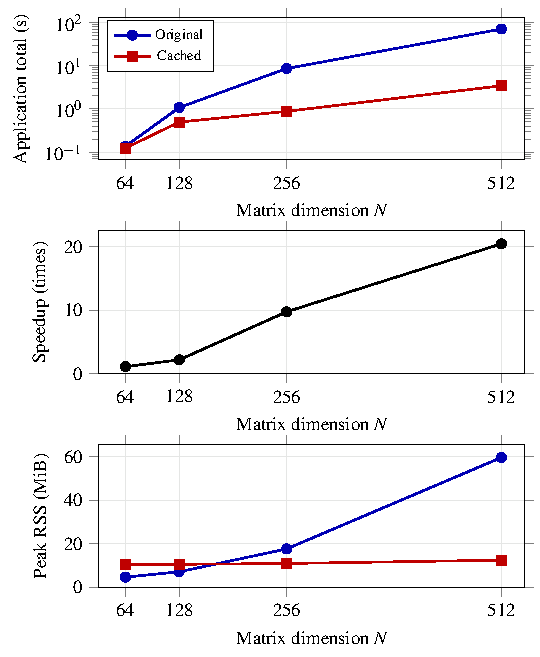
\includegraphics[width=\columnwidth]{figures/backend-comparison.pdf}
\caption{Sequential backend comparison. Times are three-run medians, speedup is
the ratio of those medians, and RSS is the largest peak across the three runs.}
\label{fig:backend-comparison}
\end{figure}

The small-input memory increase is consistent with the implementation's fixed
cost: the two binary-operation tables alone hold $2\cdot 1331^2$ two-byte IDs,
approximately 6.76~MiB, before the element catalog and other allocations.
As matrix size grows, the cached representation stores each matrix element as
a two-byte ID. This helps explain the observed reversal in RSS; these figures
do not establish a precise break-even dimension.

The product executes before the determinants and shares the same cache with
them. Consequently, determinant phase timings include the effect of entries
filled earlier and are not cold-cache determinant measurements. More cache
filling during the larger product may explain why the median sum of cached
determinant times decreases from $N=128$ to $N=256$, but occupancy was not
measured. The runs were collected in a fixed backend order on one virtualized
host; three repetitions at each size do not establish assignment-scale or MPI
performance.

\subsection{Cached Function-Level Profile}
The cached workload at $N=256$ was profiled separately with the same optimization
and gprof instrumentation described in Section~\ref{sec:original-profile}.
Ten fresh-process profiles were combined to increase the sample count; the
reported call counts and sampled seconds are totals across all ten executions.
The flat profile accounted for 7.82~s of sampled self time at a 0.01~s sampling
interval. Fig.~\ref{fig:cached-profile} shows the largest reported shares:
matrix multiplication 75.20\%, determinants 13.81\%, and polynomial division
8.70\%. Division remains present because cache misses use original arithmetic.

\begin{figure}[tb]
\centering
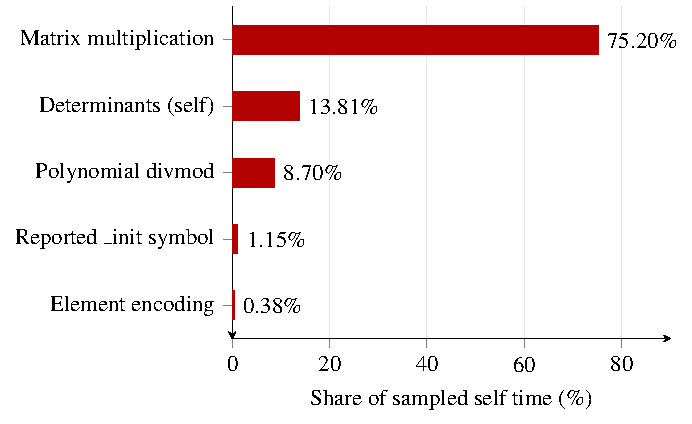
\includegraphics[width=\columnwidth]{figures/cached-profile.pdf}
\caption{Reported sampled self-time shares from ten instrumented, fresh-process
cached runs at $N=256$. Inlined arithmetic is attributed to its caller.}
\label{fig:cached-profile}
\end{figure}

These shares are relative to the sampled time of the cached profile, not a
comparison of absolute costs with Fig.~\ref{fig:original-profile}. Inlining
and sampling affect attribution~\cite{gcc-inline,gprof-sampling}; timing
speedups come from the separate uninstrumented repetitions. The profile's
19,085,010 recorded division calls are summed over ten runs and do not count
operations that were inlined.
